% Support-vector machine -- Person 3 (Yunis Allahverdi)
\subsection{Support-vector machine (from scratch)}
We implement a soft-margin linear SVM in NumPy and train it in the
primal with the Pegasos stochastic sub-gradient method~\cite{pegasos}.
Labels $\{0,1\}$ (standard, premium) are mapped to $y_i\in\{-1,+1\}$ and
the objective is
\begin{equation}
  J(\mathbf{w},b)=\tfrac{\lambda}{2}\big(\lVert\mathbf{w}\rVert^{2}+b^{2}\big)
  +\tfrac{1}{n}\sum_{i=1}^{n}\max\!\big(0,\,1-y_i(\mathbf{w}^{\top}\mathbf{x}_i+b)\big).
\end{equation}
The bias is handled as a weight on a constant feature, so it is
regularised together with $\mathbf{w}$; this is the variant suggested
in the project brief and matches the intercept treatment of
\texttt{LinearSVC}. At step $t$ we draw a mini-batch $A_t$ of $k$
examples, set $\eta_t=1/(\lambda t)$, and update
\begin{equation}
  \mathbf{w}\leftarrow(1-\eta_t\lambda)\,\mathbf{w}
  +\frac{\eta_t}{k}\sum_{i\in A_t^{+}}y_i\mathbf{x}_i ,
\end{equation}
where $A_t^{+}=\{i\in A_t: y_i(\mathbf{w}^{\top}\mathbf{x}_i+b)<1\}$ are
the points with an active hinge; $b$ follows the same rule. After each
step $(\mathbf{w},b)$ is projected onto the ball of radius
$1/\sqrt{\lambda}$, which contains the optimum~\cite{pegasos}. The
returned model is the average of the iterates over the final epoch, as in
averaged Pegasos~\cite{pegasos}: with a small $\lambda$ the step
$1/(\lambda t)$ is large and the last iterate fluctuates, which moved the
decision threshold of the RFF model between runs before we added
averaging. Setting
$k=n$ gives the full-batch sub-gradient method. The learning-rate
schedule is a hyperparameter (Pegasos $1/(\lambda t)$, $\eta_0/\sqrt{t}$,
or constant), as are $\lambda$, the number of epochs and $k$. The
objective is recorded after every epoch. All features are standardised
with training-set statistics, since the hinge loss is scale-sensitive.

After training we report $\lVert\mathbf{w}\rVert$, the margin width
$2/\lVert\mathbf{w}\rVert$, and the support vectors, defined as the
training points with $y_i(\mathbf{w}^{\top}\mathbf{x}_i+b)\le 1$.
Because our objective is exactly $\lambda$ times the
\texttt{LinearSVC} objective with $C=1/(\lambda n)$, the two solvers can
be compared directly: on a toy problem our solver reaches the same
objective value as \texttt{LinearSVC} and agrees on every prediction
(\texttt{tests/test\_svm.py}).

\paragraph{Non-linear extension}
We use random Fourier features (RFF)~\cite{rff} rather than kernelised
Pegasos. RFF maps $\mathbf{x}$ to
$\phi(\mathbf{x})=\sqrt{2/D}\cos(W^{\top}\mathbf{x}+\mathbf{c})$ with
$W_{jk}\sim\mathcal{N}(0,2\gamma)$ and $c_k\sim\mathcal{U}(0,2\pi)$, so
that $\phi(\mathbf{x})^{\top}\phi(\mathbf{z})\approx
\exp(-\gamma\lVert\mathbf{x}-\mathbf{z}\rVert^{2})$, and then runs the
same linear Pegasos solver on $\phi(\mathbf{x})$. Kernelised Pegasos
needs a coefficient per training example and kernel evaluations against
all of them, i.e.\ $O(n^{2})$ time per epoch, which is impractical on
tens of thousands of listings; RFF costs $O(nD)$ and reuses the tested
linear code. Our tests confirm that the RFF inner product approximates
the RBF kernel and that RFF-Pegasos separates concentric circles that
the linear model cannot.

\paragraph{SVM tuning protocol}
All SVM choices are made on the validation split only. For the linear
model we sweep $\lambda\in[10^{-6},10^{-1}]$ (11 log-spaced values,
20 epochs, batch 64) and pick the value with the highest validation F1.
For RFF we search $\gamma\in\{0.25,0.5,1,2,4\}/d$ and
$\lambda\in\{10^{-5},10^{-4},10^{-3}\}$ at $D=300$, then vary
$D\in\{100,300,1000\}$ and keep the smallest $D$ within $0.005$ F1 of
the best, because RFF memory grows as $O(nD)$. Sweeps use at most
20{,}000 training rows; final models are refit on the full training set.

\paragraph{Baselines and uncertainty}
The scikit-learn baselines minimise the same objectives as ours:
\texttt{LinearSVC} (hinge loss, $C=1/(\lambda n)$),
\texttt{SGDClassifier} (hinge loss, $\alpha=\lambda$) and \texttt{SVC}
with an RBF kernel ($C=1/(\lambda n)$, same $\gamma$ as RFF), each
inside a \texttt{Pipeline} with \texttt{StandardScaler}. Uncertainty is
reported as mean $\pm$ std over 5-fold stratified cross-validation on
train+validation, with the scaler refit inside each fold, together with
mean fit and predict times. Because \texttt{SVC} scales quadratically
with $n$, it is trained on a 5{,}000-row subsample per fold; this is
stated next to its numbers. Test-set metrics come from a single fit on
the training split.

\begin{figure}[t]
  \centering
  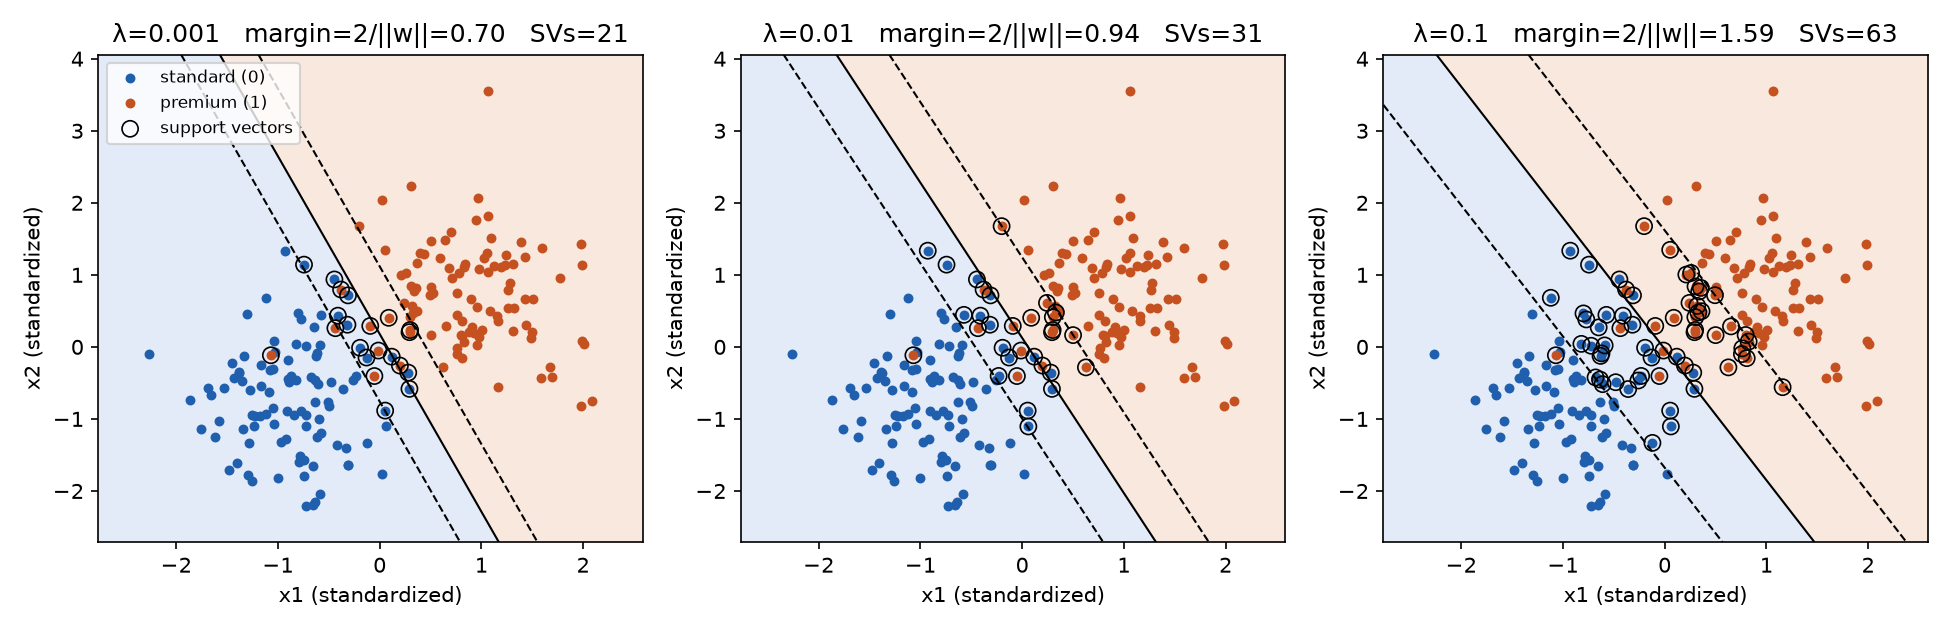
\includegraphics[width=\linewidth]{figures/fig_svm_margin_2d.png}
  \caption{Linear Pegasos on a 2-D toy problem. Larger $\lambda$ gives a
  smaller $\lVert\mathbf{w}\rVert$, a wider margin (dashed) and more
  support vectors (circled).}
  \label{fig:svm_margin}
\end{figure}

\begin{figure}[t]
  \centering
  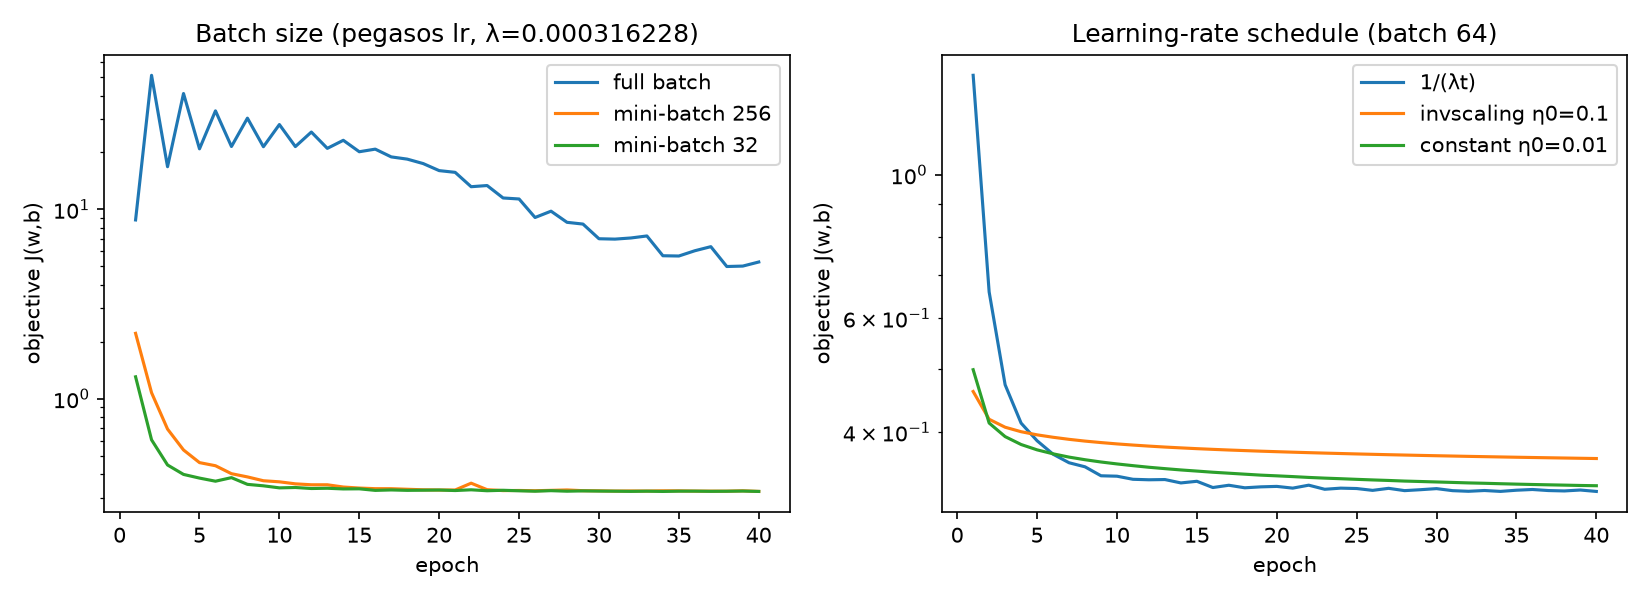
\includegraphics[width=\linewidth]{figures/fig_svm_objective.png}
  \caption{Training objective per epoch for the chosen $\lambda$: effect
  of batch size (left) and learning-rate schedule (right).}
  \label{fig:svm_objective}
\end{figure}

\begin{figure}[t]
  \centering
  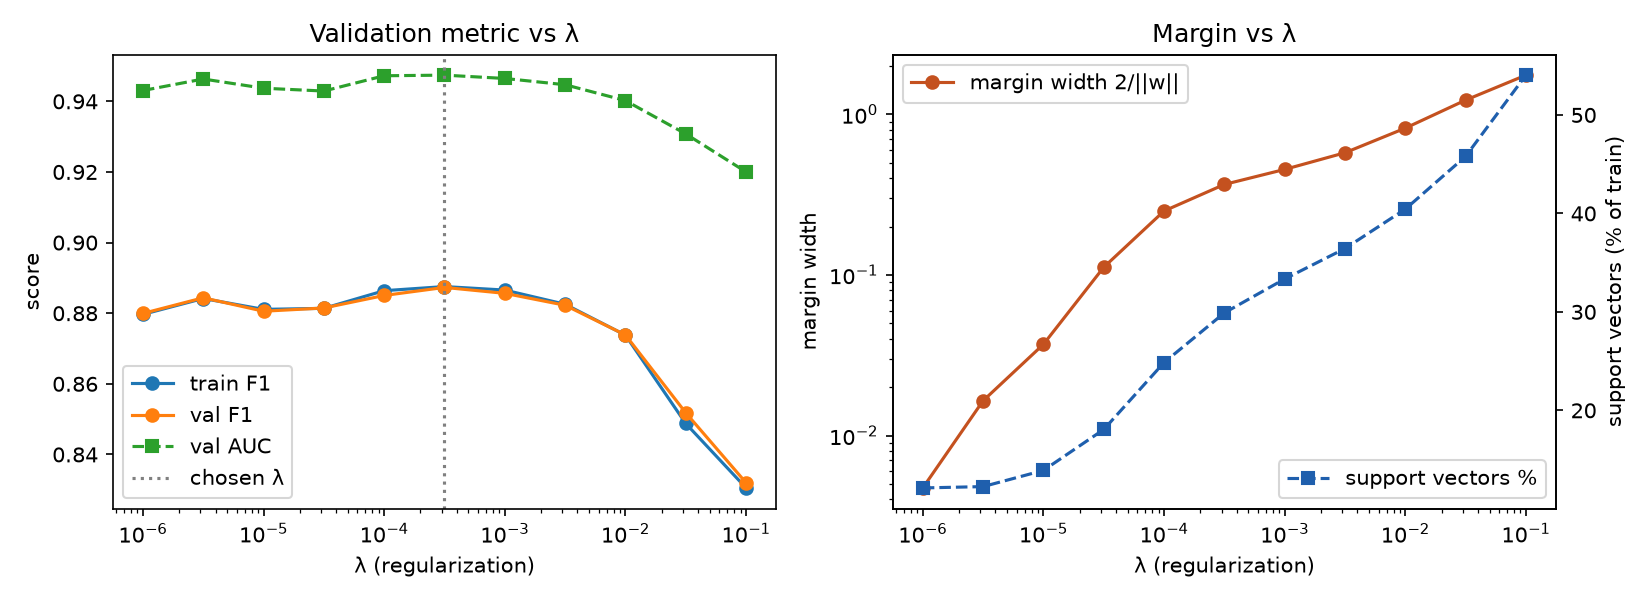
\includegraphics[width=\linewidth]{figures/fig_svm_lambda_sweep.png}
  \caption{$\lambda$ sweep: validation F1/AUC (left) and margin width
  and share of support vectors (right). The dotted line marks the
  chosen $\lambda$.}
  \label{fig:svm_lambda}
\end{figure}

\begin{figure}[t]
  \centering
  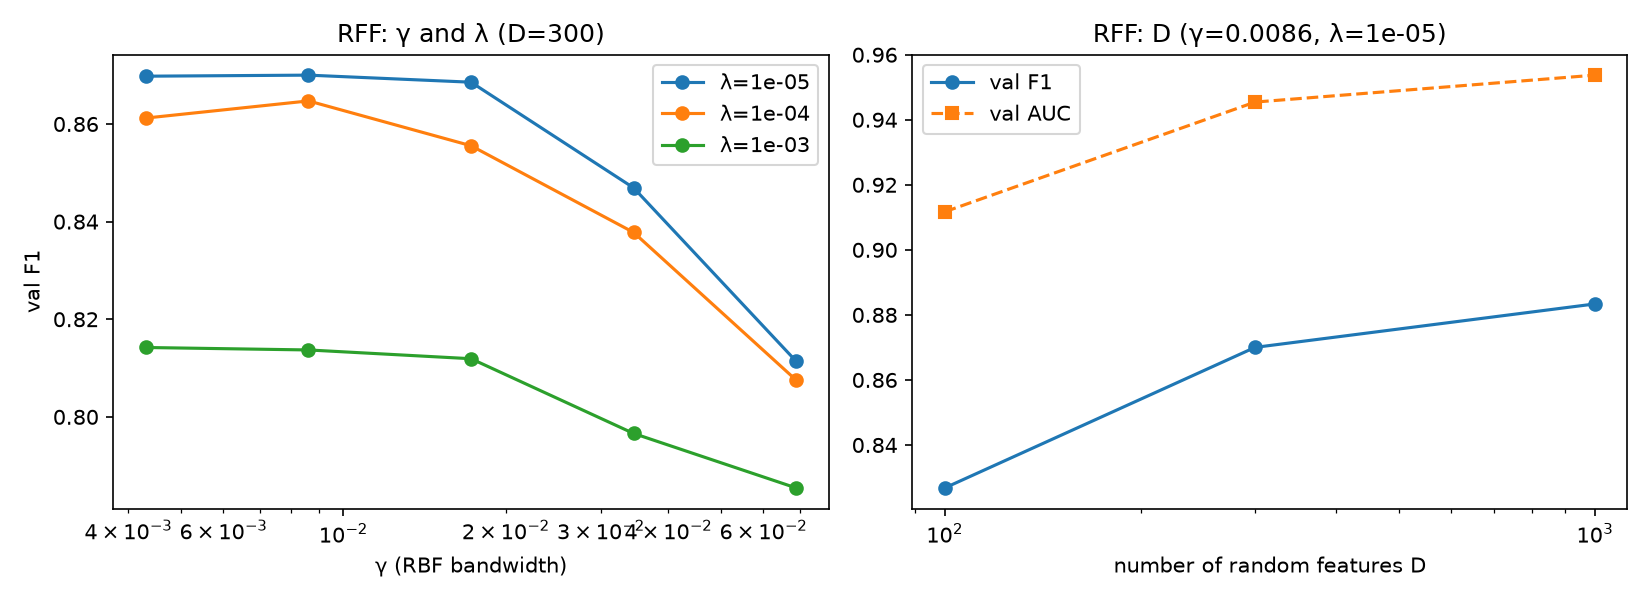
\includegraphics[width=\linewidth]{figures/fig_svm_rff_sweep.png}
  \caption{Random Fourier features: bandwidth $\gamma$ and $\lambda$
  (left) and number of random features $D$ (right).}
  \label{fig:svm_rff}
\end{figure}

\paragraph{Error analysis}
Inspecting the linear SVM on the validation split, the error rate falls
steadily with the distance $|\log(\text{price}/\text{threshold})|$ between a
listing's price and the tier threshold (Fig.~\ref{fig:svm_errors}): it is
highest for listings priced close to the boundary, where a small price
difference flips the label. The largest positive and negative weights
of the linear model (Fig.~\ref{fig:svm_weights}) show which standardised
features push a listing towards the premium tier.

\begin{figure}[t]
  \centering
  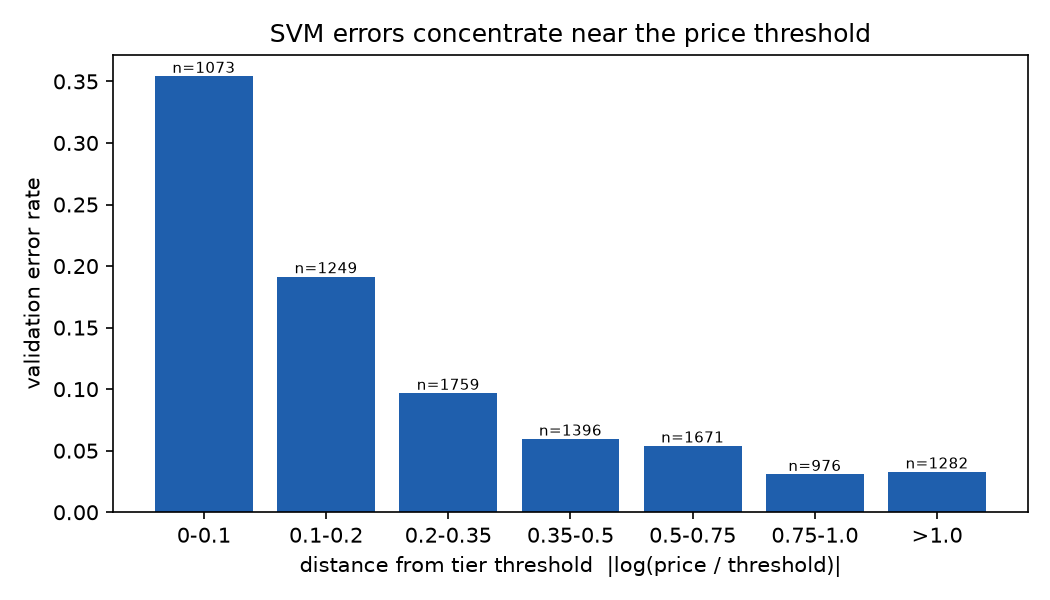
\includegraphics[width=\linewidth]{figures/fig_svm_errors.png}
  \caption{Validation error rate of the linear SVM by distance from the tier threshold.}
  \label{fig:svm_errors}
\end{figure}

\begin{figure}[t]
  \centering
  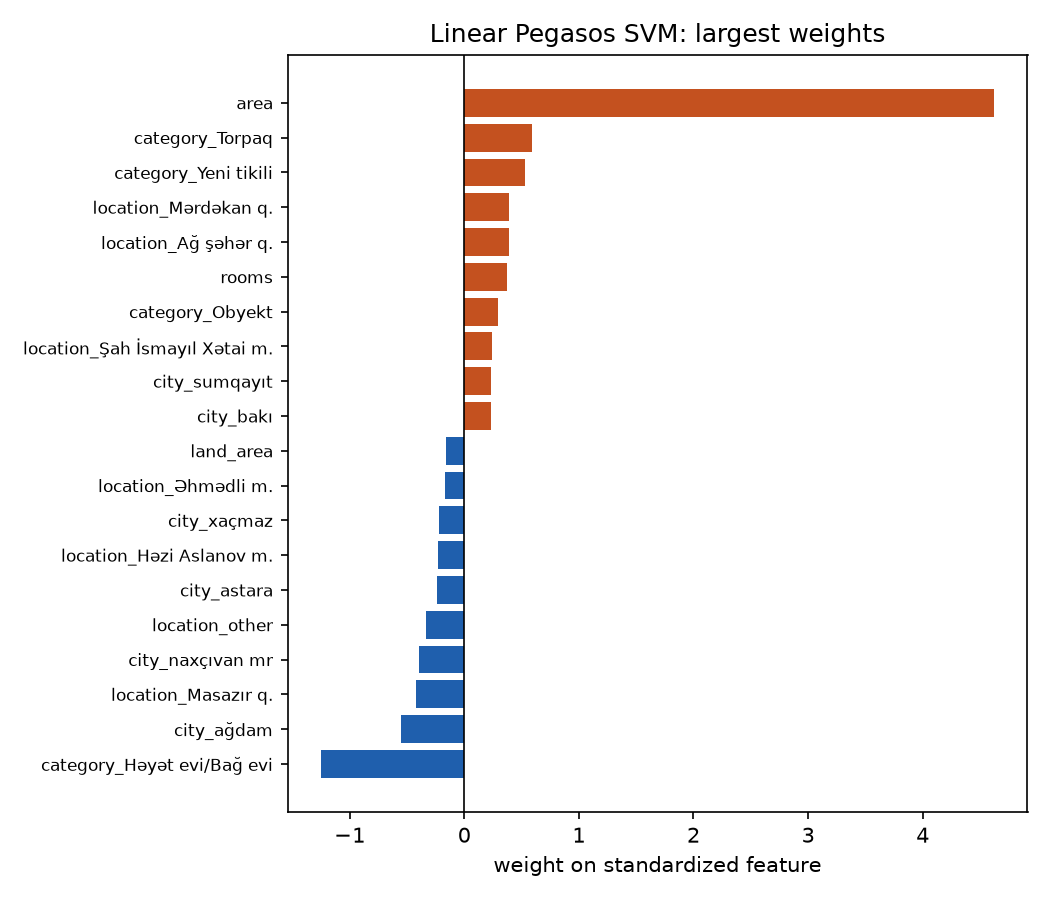
\includegraphics[width=0.85\linewidth]{figures/fig_svm_weights.png}
  \caption{Largest weights of the linear Pegasos SVM (standardised features).}
  \label{fig:svm_weights}
\end{figure}
